\documentclass[tikz]{standalone}

\usetikzlibrary{mindmap}

\begin{document}
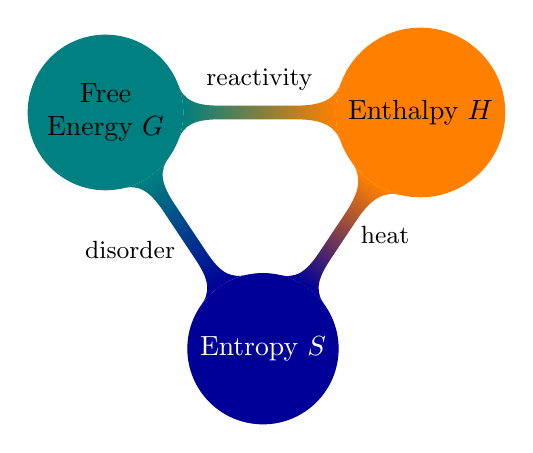
\begin{tikzpicture}[align=center]

  \node (enthalpy) at (2, 0) [concept, concept color=orange] {Enthalpy $H$};

  \node (free-energy) at (-2, 0) [concept, concept color=teal] {Free\\Energy $G$};

  \node (entropy) at (0, -3) [concept, concept color=blue!60!black, text=white] {Entropy $S$};

  \path (enthalpy) to[circle connection bar switch color=from (orange) to (teal)] node[above=1ex, font=\small] {reactivity} (free-energy);

  \path (entropy) to[circle connection bar switch color=from (blue!60!black) to (orange)] node[right=1ex, font=\small] {heat} (enthalpy);

  \path (free-energy) to[circle connection bar switch color=from (teal) to (blue!60!black)] node[below left=0, font=\small] {disorder} (entropy);

\end{tikzpicture}
\end{document}
